%%%%%%%%%%%%%%%%%%%%%%%%%%%%
% SECTION                  %
%%%%%%%%%%%%%%%%%%%%%%%%%%%%
\vspace{1em}

Sur le territoire de la Principauté, l'AMSN doit épauler la sécurité numérique de plusieurs dizaines d'administrations publiques et d'entreprises classées OIV, représentant autant de réseaux à superviser avec des milliers d'utilisateurs et d'appareils connectés.
L'Agence ne peut mener à bien cette mission qu'avec la coopération de ces acteurs, qui l'autorisent à placer des sondes en amont, et parfois à l'intérieur, de leurs réseaux. Toutes les actions des utilisateurs qui entrent et sortent des réseaux supervisés passent par les sondes qui disposent d'un IDS, en l'occurrence ici Suricata, lequel contrôle le contenu de ces flux réseau à l'aide de règles de détection qui, si elles sont déclenchées, génèrent des événements de sécurité gérés par le SOC-MC.

\begin{figure}[h]%
    \center%
    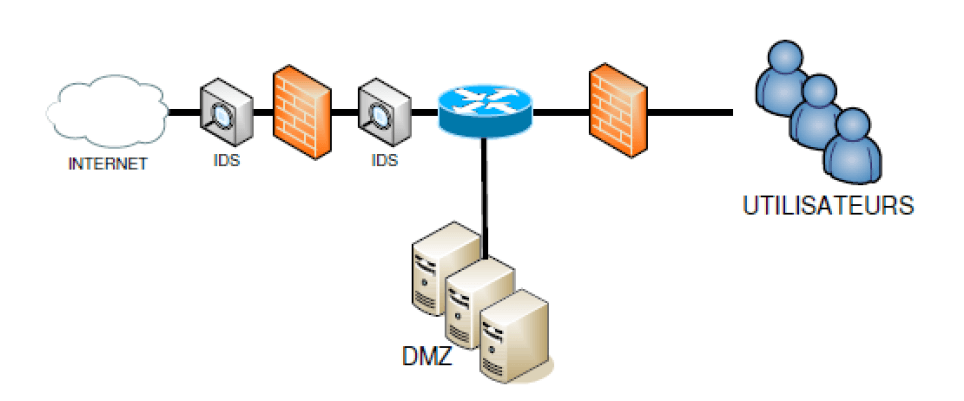
\includegraphics[width=1\textwidth]{assets/reseau.png}
    \caption[Exemple de disposition de sonde IDS dans le réseau d'un OIV (source:\href{https://blogger.googleusercontent.com/img/b/R29vZ2xl/AVvXsEhz0rffx8tqoJRqjF0Hf3LAERS8e7tpmQVnPzlBITzud8iMUOh63zfDIyLKLXnQprLLNAycblYb02W3Y4004q3ruHhdZ3T9Dy7KTMyydsLMRjR2UGkzQ6hIOcwM8DiSLeLp0pZeyyCt5CDl/s1600/Capture.PNG}{eventus-networks.blogspot.com})]{Exemple de disposition de sonde IDS dans le réseau d'un OIV}\label{fig:test}
\end{figure}

\vspace{1em}

Ces règles sont créées à partir d'indicateurs de compromission (IOC) établis en interne ou grâce à des renseignements externes provenant de CERT partenaires (comme le CERT-FR de l'ANSSI) ou d'agences privées de cyber-renseignement (également appelées CTI). Les règles générées par ces partenaires externes posent souvent des problèmes :\\

\begin{itemize}[itemsep=0.75em]
    \item[•] Les règles générées sont fréquemment génériques et mal adaptées, engendrant trop d'événements inutiles ou redondants dans le réseau où elles sont mises en œuvre (ces réseaux sont tous basés sur des technologies différentes).
    \item[•] Les renseignements extérieurs ne proviennent que d'une poignée d'acteurs, et l'agence ne peut être certaine de pouvoir détecter toutes les menaces existantes à l'état de l'art.\\
\end{itemize}

\newpage

Ces difficultés de l'AMSN sont communes aux institutions publiques et aux entreprises qui doivent remplir les mêmes missions. Cela légitime la problématique posée : "Comment mettre en place un outil automatisé de génération de règles de détection d’intrusion ?"\\

Pour aborder cette problématique, il faut se poser les questions suivantes :
\vspace{0.5em}
\begin{itemize}[itemsep=0.5em]
    \item[•] Où recueillir le cyber-renseignement nécessaire à l'établissement des IOC ? Et comment évaluer la qualité de ces renseignements ?
    \item[•] Comment générer des règles automatiquement à partir de ces IOC ?
    \item[•] Comment s'assurer que ces règles soient aussi pertinentes que possible pour la partie prenante supervisée ?\\
\end{itemize}

Mes travaux, menés dans le cadre de l'AMSN, visent à répondre à cette problématique et à fournir une solution capable de résoudre les problèmes posés à l'Agence ou à tout autre acteur similaire oeuvrant pour la protection des systèmes d'information.